%----------------------------------------------------------------------------
\chapter{Technológiai ismertető}
%----------------------------------------------------------------------------

\section{Programozási paradigmák fejlődése}

Napjaink nagyméretű, sokszor többmilliónyi kódsorból álló programrendszereinek kifejlesztése elképzelhetetlen előzetes programtervezés nélkül.
A különféle tervezésmódszertanok nyomot hagytak a szoftverek tervezési módszerein is.
Egyik híres módszertan a Barry Boehm által 1988-ban publikált Spirál modell, melyben a fejlesztés szokásos fázisai -- követelmény specifikáció, feladatelemzés, architekturális tervezés, algoritmikus tervezés, implementálás, tesztelés -- mellett megjelenik az élet folytonosságát kifejező, magasabb szinten való ismétlődése a fejlesztési lépéseknek.
A különböző szoftverfejlesztési paradigmák -- moduláris, strukturális, objektum orientált, komponens alapú, aspektus orientált, generikus (template alapú), evolúciós, intencionális, multiparadigmás -- nélkül a nagyméretű, korszerű programrendszerek előállítása lehetetlen volna.
A modern szoftverfejlesztést támogató -- \gls{CASE}, computer-aided software engineering -- eszközök egyik ismert tagja az említett tervezési folyamat első lépéseit támogató Unified Modeling Language (\gls{UML}).  
A fejlett szoftverparadigmák mindegyike kiemelten kezeli a modellezés különböző szintjeinek gépi támogatását.
Ismert tény, hogy az adott programnyelven történő implementálás időigényének nagyságrendjébe esik a tesztelés és az előzetes rendszertervezés időigénye is, így ezek automatizálásának szándéka érthető.

%----------------------------------------------------------------------------

\section{A modellezés előnyei}

A modell definíciószerűen egy rendszer, elmélet, vagy jelenség leírása, mely rendelkezik annak ismert, vagy kikövetkeztetett tulajdonságaival és a jellemzői további vizsgálatára használható \cite{dict:Model}. 
A szoftverrendszerek tervezésénél többféle modellt alkalmaznak:
\begin{itemize}
	\item adatszerkezeti modell (objektummodell, osztályhierarchia, öröklődés, stb.)
	\item funkcionális modell (adatforrások, -tárolók, -nyelők, -folyamok)
	\item dinamikus modell (állapotok, események, kommunikáció) \cite{Kondorosi07}.
\end{itemize}
Az ezen modelleken alapuló nézetek és diagramok -- osztályhierarchia, külső felhasználók, objektumok együttműködése, tevékenységek, események időbelisége, objektumok állapota, rendelkezésre álló szoftver- és hardver erőforrások -- nélkül a tervezés nagy rendszerek esetében áttekinthetetlen, a rendszer implementálás előtti tesztelése, viselkedésének elemzése, idő- és költségbecslések elvégzése kivitelezhetetlen. 
A modellezés fejlődése a szoftverfejlesztésben 2001-re elvezetett a \emph{model-driven architecture} (\gls{MDA}) szoftvertervezési metodológia és eszközrendszer kifejlődéséhez, mely az Object Management Group (\gls{OMG}) nevéhez fűződik \cite{wiki:ModelDrivenArchitecture}.

%----------------------------------------------------------------------------

\section{Platformfüggetlen szoftvermodellezés}

Az \gls{MDA} metodológia a szoftverrendszer funkcionalitását platformfüggetlen modell (\gls{PIM}, platform-independent model) alkalmazásával, megfelelő doménspecifikus leírónyelv (\gls{DSL}, domain-specific language) segítségével definiálja.
Egy konkrét szoftverfejlesztési platform megadása után a platformfüggetlen modellt lefordítja az adott, konkrét platformon működő modellre (\gls{PSM}, platform-specific model).
A modell-vezérelt architektúrához (\gls{MDA}) kapcsolódik többek között a jól ismert \gls{UML} rendszermodellező nyelv és az \gls{XMI} (XML Metadata Interchange) metaadatok XML-alapú cseréjét biztosító szabvány is \cite{wiki:ModelDrivenArchitecture}. 
Az \gls{MDA} által felhasznált eszközök az alábbi kategóriákba sorolhatóak:
\begin{itemize}
	\item \emph{szerkesztő eszközök} (creation tools) modellek létrehozására, szerkesztésére
	\item \emph{elemző eszközök} (analysis tools) a modellek teljességének, konzisztens szerkezetének, hibamentességének ellenőrzésére, szoftvermetrikák számítására
	\item \emph{transzformációs eszközök} (transformation tools) meglévő modellek más modellekbe alakításhoz, vagy programnyelvekre fordításhoz, dokumentáláshoz
	\item \emph{kompozíciós eszközök} (composition tools) több forrásmodell egy modellé egyesítéséhez
	\item \emph{tesztelő eszközök} (test tools) a modellek teszteléséhez
	\item \emph{szimulációs eszközök} (simulation tools) a modell által leírt rendszer működésének szimulálásához
	\item \emph{metaadat menedzselő eszközök} (metadata management tools) különböző modellek közti általános kapcsolatok és metaadatok -- pl. létrehozó, létrehozási idő, stb. -- kezelésére
	\item \emph{visszafejtő eszközök} (reverse engineering tools) idejétmúlt modellek vagy más információhordozók teljes értékű modellekké alakítására.
\end{itemize}

A szakdolgozat keretében kifejlesztendő komponensek modell-lekérdezések -- melyekre szintén tekinthetünk modellként -- analízisére lesznek alkalmasak, emiatt az elemző eszközök közé tartoznak. 

%----------------------------------------------------------------------------

\section{Platform-specifikus szoftvermodellezés}

Míg az \gls{MDA} nyújtja a platformfüggetlenséggel az általános modellezés magas szintjét és az ebből eredő átjárhatóságot a platformok között, addig a konkrét alkalmazások létrehozásához az \gls{MDA}-ban készült platformfüggetlen modellt (\gls{PIM}) le kell fordítani egy adott szoftverplatformra.
Ennek a fordításnak az eredményeként a szoftvermodell valamilyen doménspecifikus környezeten áll elő, mely jelenthet pl. egy C++ nyelvi környezetet is.

A specializálódás előnyökkel és hátrányokkal is jár.
Az előnyök között említhetjük a doménspecifikus szoftvertechnológia nagyobb hatékonyságát, adott területen akár félkész megoldást nyújtó jellegét, a modellezett feladat természetéhez való jobb illeszkedést -- pl. a Prolog nyelv -- a futtatókörnyezetében -- beépítetten tartalmazz egy következtető automatát, ami szakértőrendszer alkalmazások írásakor már a megoldás fele.
Ugyanakkor a specializálódásból származnak hátrányok is: az átjárhatóság, magasabb szintű absztrakciók elvesztése, speciális programozási ismeretek iránti igény, a hordozhatóság csökkenése.
Egy közbenső szintet jelent a doménspecifikus modellezés nyelveinek (\gls{DSML}, domain-specific modeling language) alkalmazása, melyek a \gls{DSM} szoftverfejlesztési metodológia eszközeként az \gls{MDA}-tól specifikusabb, de az általános célú programozási nyelvektől (pl. C++, Java, C\#) általánosabb reprezentációs szintet képviselnek \cite{wiki:DomainSpecificModeling}.
Ezen a szinten, illetve \gls{DSML} nyelven leírva a programozási feladatot, már alkalmazhatunk automatikus kódgenerálást is, amely valamely általános programnyelvre fordítja a formális modellünket.
A \gls{DSML} nyelven való feladatleírás könnyebbsége és kisebb részletesség iránti igénye az ily módon végzett szoftverfejlesztés hatékonyságában is megmutatkozik, mely összemérhető a \gls{CASE} eszközök, illetve az \gls{UML} hatékonyságával és absztrakciós szintjével, de azoktól korszerűbb, és azoktól szélesebb körben használható.
A \gls{DSM} környezetek a magas szintű leírónyelven és az abból általános programnyelvű kódot generáló fordítón kívül általában további általánosan használt alapszolgáltatásokat is nyújtanak.
A dolgozatban a következőkben egy ilyen környezetet, az Eclipse Modeling Framework-öt (\gls{EMF}) mutatjuk be, mivel a feladatunk az EMF-IncQuery EMF-plugin keretrendszer alkalmazása lesz.
Az \gls{EMF} az Eclipse nyílt forráskódú, platformfüggetlen magas szintű szoftverfejlesztési környezet általános modellező keretrendszere.

%----------------------------------------------------------------------------

\section{Az Eclipse integrált szoftverfejlesztő keretrendszer}

Az elsősorban Java nyelven íródott Eclipse integrált fejlesztő környezet (Integrated Development Environment, IDE) alkalmas Java alkalmazások fejlesztésére, a beépített Java fejlesztési eszközöket is tartalmazó szoftverfejlesztő készletnek (Software Development Kit, SDK) köszönhetően. Hasonlít céljaiban a Microsoft Visual Studio, vagy az Embarcadero Rapid Application Development (RAD) Studio integrált többnyelvű szoftverfejlesztő környezetre [RAD Studio XE5, http://www.embarcadero.com/products/rad-studio]. Az Eclipse is az alap munkakörnyezeten kívül az igen gazdag plugin készletnek köszönhetően számtalan további programnyelven teszi lehetővé a fejlesztést. Ilyen nyelvek többek között a C++, COBOL, FORTRAN, JavaScript, Perl, PHP, Python, Erlang. Platformfüggetlenségét Linux, Mac OS X, Solaris és Windows operációs rendszereken való futtathatósága jelenti, lásd \ref{fig:EclipseIDE}. ábrát. Az Eclipse Foundation fejlesztő társaság gondoskodik a rendszeres továbbfejlesztésről és új összetevők hozzáadásáról. A legutóbbi 4.3 verzió a Kepler nevet viseli és 2013. június 26-án jelent meg, de már folyik a legújabb, Luna projekt is \cite{wiki:EclipseIDE}. 

\begin{figure}[h]
\centering
\includegraphics[width=\textwidth]{figures/eclipse-ide.png}
\caption{Eclipse fejlesztőkörnyezet Windows 7 operációs rendszeren}
\label{fig:EclipseIDE}
\end{figure}

Az Eclipse fejlesztésében a nyílt forráskódú platformjának köszönhetően számtalan projektben sok külsős szoftverfejlesztő vesz részt. Az integrált szoftverelemek felölelik a szoftverfejlesztés majd minden fázisát. A fejlesztést szolgáló projektekről az Eclipse-közösség főoldaláról elérhető Projects (\url{http://www.eclipse.org/projects/}) lapon tájékozódhatunk. A különböző fejlesztési fázisában lévő 235 fő- és alprojekt mutatja a kezdeményezés nagyságát. A fő projektek között megtaláljuk a
\begin{itemize}
	\item Data Tools Platform
	\item Eclipse Project
	\item Eclipse Modeling Project
	\item Mylyn
	\item RT
	\item SOA Platform Project
	\item Technology Project 
	\item Tools Project
	\item Eclipse Web Tools Platform Project
\end{itemize}
főágakat, melyek közül számunkra a dolgozat témája miatt az Eclipse Modeling Project főág a benne található Eclipse Modeling Framework (EMF) és EMF-IncQuery alprojektek miatt, valamint az utóbbihoz kapcsolódó Xtext és VIATRA2 projektek miatt a legfontosabb.

%----------------------------------------------------------------------------

\section{A PDE - Plugin Development Environment alprojekt}

Az Eclipse Projekt célja, a nyílt szoftverkódú, robosztus, általános célú, kereskedelmi színvonalú ipari platform kidolgozásához magas szinten integrált eszközök és kövér kliens alkalmazások fejlesztése. Ennek eléréséhez a PDE - Plugin Development Environment nyújt támogatást Eclipse pluginok, kódrészletek, sajátosságok, különféle kiegészítések, szoftverkomponensek kifejlesztésének lehetővé tétele és egyéb támogatás formájában. Az alprojekt továbbá az OSGI tooling keretében ideális környezetet nyújt a komponens programozáshoz is a plugin fejlesztésen túl. Az új összetevők rendszerint az eszközpaletta új gombjával illeszthetők a fejlesztett alkalmazásba.
A PDE projekt Build, UI és API alrészeiben kifejlesztett funkcionalitások segítették a BME Villamosmérnöki és Informatikai Karán működő Hibatűrő Rendszerek Kutatócsoportot az EMF-IncQuery keretrendszer kifejlesztésében, mely modell-lekérdezések deklaratív módon történő definiálását és hatékony végrehajtását teszi lehetővé.

%----------------------------------------------------------------------------

\section{Az Eclipse Modeling Framework} \cite{VogelEMF}
Az Eclipse Modeling Framework (EMF) adatszerkezetek, domének modellezésére szolgáló plugin, mely 2002-től áll a szoftverfejlesztők rendelkezésére. Modell-vezérelt szoftverfejlesztést tesz lehetővé, képes a modellezett adatszerkezet osztályok Java kódjának generálására is. Ily módon könnyen áttekinthető vizuális támogatással és grafikus szerkesztővel hozhatunk létre robusztus, nagyméretű adatrendszer modelleket, melyekből a közvetlen kódgenerálás is megoldott. Az EMF előnyei között említendő a csoportmunka támogatása is. Az adatszerkezetek modellezésére vonatkozó ajánlás azok elkülönítése a programkódtól, ily módon csak adattagokat tartalmazó osztályok definiálása. 
Az EMF megkülönbözteti az adatmodell modelljét, azaz az adatmodell szerkezetét leíró meta-modellt az aktuális modelltől, mely a meta-modell, mint osztály egyedeként fogható fel. 
Az EMF modellező széles elterjedségét magyarázza a magasszintű modellezés kivitelezésének könnyű volta, az erős integráltsága az Eclipse alá, továbbá az automatikus kódgenerálás. Számtalan alkalmazása közül megemlítendő több Eclipse projektben való felhasználása.

A továbbiakban mélyebben elemezzük az EMF szerkezetét és lehetőségeit az \url{http://www.eclipse.org/modeling/emf/docs/} weboldalon található áttekintő cikkek feldolgozása révén.

Metamodellből kettő található az EMF-ben:
\begin{itemize}
	\item Ecore metamodell és 
	\item Genmodel metamodell.
\end{itemize} 
Az Ecore metamodell a definiált osztályokról tartalmaz információt, míg a Genmodel a Java kód generálásához tartalmaz járulékos adatokat, mint pl. fájlnevet és elérési utat, valamint a kódgenerálás vezérlő paraméterét. Az Ecore metamodell különféle elemek definiálását teszi lehetővé:
\begin{itemize}
	\item EClass: attribútumokat és/vagy hivatkozásokat tartalmazó osztály
	\item EAttribute: névvel és típussal rendelkező attribútum
	\item EReference: két osztály közötti kapcsolat egyik végét reprezentálja. Egy flag-gel jelzi, ha reprezentál egy tartalmazást és egy hivatkozási osztályt, amelyre mutat.
	\item EDataType: adattípus, pl. int, float, java.util.Date.
\end{itemize}

Az Ecore metamodell felépítését a \ref{fig:EcoreStruct}. ábra mutatja.

\begin{figure}[h]
\centering
\includegraphics[width=\textwidth]{figures/ecore-metamodel-struct.png}
\caption{Ecore meta-modell szerkezete}
\label{fig:EcoreStruct}
\end{figure}

Az Ecore meta-modell fő elemei a \ref{fig:EcoreStruct}. ábra kontextusába helyezve a következők \cite{EMFFundamentals}: 
A gyökér objektum egy EObject elem, ebbe tartoznak az EPackage csomagok, melyek egyszerre kezelendő osztályokból (EClass és EDataType) épülnek fel. A class szinten EClass elemek reprezentálják a modellezett osztályokat, melyek a nevükből és EAttribute és/vagy EReference elemekből állnak. Az attribútumoknak neve és típusa is van, míg a referenciák egyirányú bináris kapcsolatot modelleznek, nevük van és megadják a hivatkozott osztály típusát és a tartalmazásjelző flag-et. Az adattípust az EDataType elem adhatja meg.  

Az alkalmazások konkrét adatmodelljei az Ecore meta-modell egyedei. A \ref{fig:DataModelWithXMI}. ábra mutat egy konkrét példát egy alkalmazás adatmodelljére.

\begin{figure}[h]
\centering
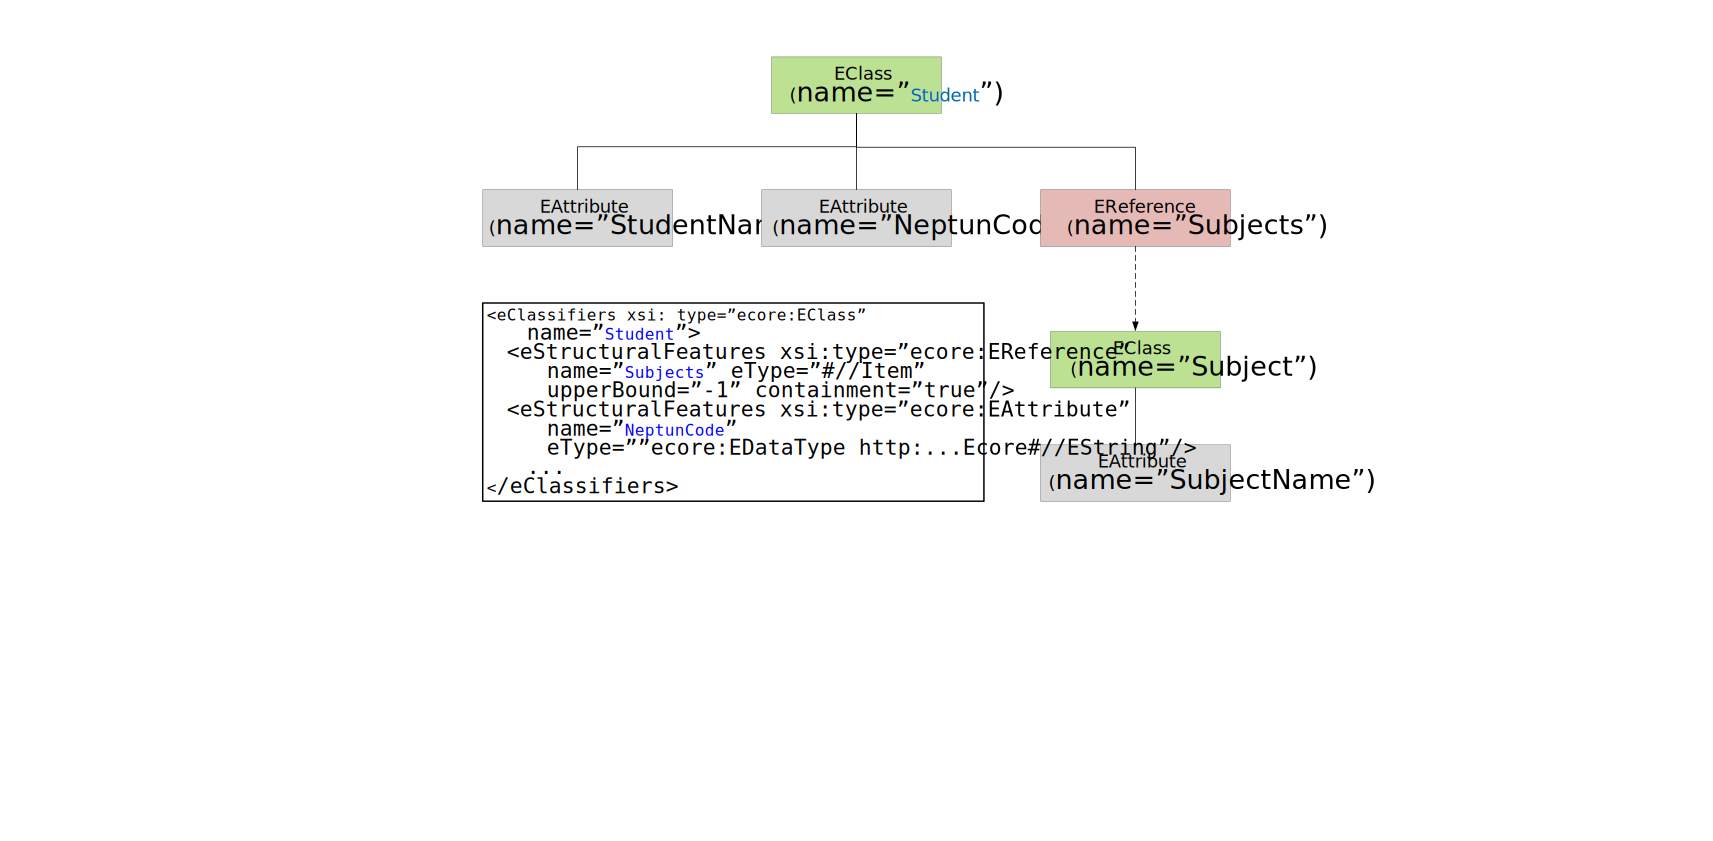
\includegraphics[width=\textwidth]{figures/datamodel-example-with-xmi-desc.png}
\caption{Alkalmazás adatmodell példa, XMI formátumú megadással}
\label{fig:DataModelWithXMI}
\end{figure}

Az EMF modell lényegében az UML Osztály Diagram nézetének egy részhalmaza \cite{EMFFundamentals}.
Az EMF modellek az alábbi módokon is megadhatók:
\begin{enumerate}
	\item Java Interfaces
	\item UML Class Diagram
	\item XML Schema
\end{enumerate}
alakjában. A modellimport és a kódgenerálás lehetőségeit a \ref{fig:ModelImportAndCodegen}. ábrán láthatjuk \cite{EMFFundamentals}.

\begin{figure}[h]
\centering
\includegraphics[width=\textwidth]{figures/model-import-and-codegen.png}
\caption{Modell import és kódgenerálás}
\label{fig:ModelImportAndCodegen}
\end{figure}

A kódgenerálás oda-vissza működik, Ecore modell generálható annotált Java interfészekből \cite{MasteringEMF}. A generált kód tartalmazza az interfészt és az osztály implementációt, pl. a \ref{fig:DataModelWithXMI}. ábra szerinti modell esetén a következő formában:

\begin{lstlisting}
public interface Student extends EObject
{
    String getStudentName();
    void setStudentName(String value);
    String getNeptunCode();
    void setNeptunCode(String value);
    EList<Subject> getSubjects();
}
\end{lstlisting}
\begin{lstlisting}
public class StudentImpl extends EObjectImpl
    implements Student
{
    ...
}
\end{lstlisting}
A programkód tartalmazza a getter/setter elérőfüggvényeket az attribútumokhoz és a referenciákhoz.

Az EMF meta-modell létrehozását az \ref{fig:EcoreDiagramEditor}. ábra szerinti grafikus szerkesztő segíti.

\begin{figure}[h]
\centering
\includegraphics[width=\textwidth]{figures/ecore-diag-editor.png}
\caption{Ecore grafikus modellszerkesztő}
\label{fig:EcoreDiagramEditor}
\end{figure}

Egy példát egy adatszerkezetre \cite{VogelEMF} alapján a \ref{fig:EcoreKarateMetaModel}. ábra mutat.

\begin{figure}[h]
\centering
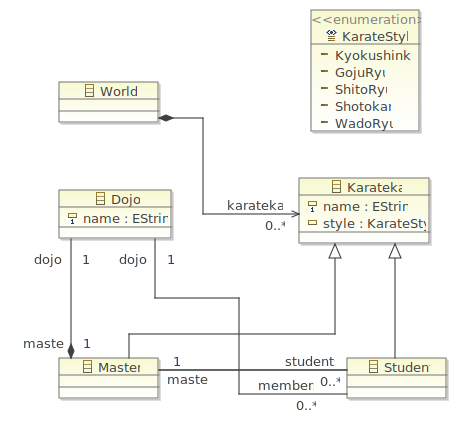
\includegraphics[width=\textwidth]{figures/ecore-karate-metamodel-diag.png}
\caption{Példa Ecore meta-modellre (Karate meta-model)}
\label{fig:EcoreKarateMetaModel}
\end{figure}

A dolgozatban kulcsszerepet játszó Eclipse Modeling Framework (\gls{EMF}) bemutatásának összefoglalásaként a következőket emelhetjük ki \cite{EMFFundamentals}:
Az \gls{EMF} a legkézenfekvőbb modellező eszköz a Java környezet számára.
Az alkalmazás belső modelljére épít, nem szükséges más magas szintű modellező eszköz.
A modellezést és a programozást keverten is képes kezelni növelve ezáltal mindkettő hatásfokát.
A szoftverfejlesztés termelékenységét növeli és megkönnyíti az integrációt.
Mindezek alapján az Eclipse modell alapú fejlesztésének és adatintegrációjának az alapja. 

A feladatkiírás szerint az \gls{EMF}-re épülő, a Méréstechnika és Információs Rendszerek Tanszéken kidolgozott, modell-lekérdezések végrehajtására alkalmas EMF-IncQuery keretrendszerben kell vizsgálatokat végeznem, ezért a következőkben a keretrendszert ismertetem.

%----------------------------------------------------------------------------

\section{EMF-IncQuery}

A fejezet célja az EMF-IncQuery használatának és a lekérdező nyelv felépítésének bemutatása, továbbá a feladatkiírás első pontjának megfelelően az EMF modellek lekérdezésének az EMF-IncQuery rendszerrel történő elvégzésének bemutatása.
A keretrendszert a \url{http://incquery.net/incquery}\todo{ezt hogy kéne hivatkozni?} forrás alapján ismertetem.

Az EMF-IncQuery EMF modelleken végzendő deklaratív lekérdezések definiálására alkalmas keretrendszer.
Fontos jellemzője, hogy a definiált lekérdezéseket kézi programírás nélkül, hatékonyan hajthatjuk végre.
A lekérdező nyelv a gráfmintázatok keresésének módszerét alkalmazza, amely tömör és könnyű eljárás komplex szerkezeti modell-lekérdezések definiálására és végrehajtására.
A kiemelkedő lekérdezési hatásfokot azáltal nyújtja, hogy inkrementális gráfkeresési technikákat alkalmaz.
Ennek köszönhetően a keresés még milliós nagyságrendű elemszám mellett is gyors.
Hatékony egyed-listázás, számbavétel és visszafelé történő navigálás jellemzi, mely az EMF API-val sokszor ütközik gondba.
Az újabb verzió képes származtatott sajátosságok, mint pl. virtuális attribútumok és referenciák kiértékelésére is.

\begin{figure}[h]
\centering
\includegraphics[width=\textwidth]{figures/emf-incquery-structure.png}
\caption{Az EMF-IncQuery felépítése}
\label{fig:EMFIncQueryStructure}
\end{figure}

A \ref{fig:EMFIncQueryStructure}. ábra mutatja az EMF-IncQuery felépítését \cite{Bergmann-TOOLS-2012}.
A megadott lekérdezésen (Query specification) alapulva mintaellenőrző pluginok generálódnak (Generated pattern matcher), melyek könnyen integrálhatók egy meglévő Eclipse-alapú alkalmazásba (Application, Application code).
A lekérdezés megadását Xtext 2-alapú szerkesztő támogatja, amely fejlett szintaxis kiemeléssel, kódkiegészítéssel és formula ellenőrzéssel rendelkezik.
Ezek a pluginok az EMF-IncQuery API-n keresztül elérik a rendszer belső funkcionalitását.
Az API-ban a Validation Engine, validáló motor körbeveszi az EMF Validációs Szolgáltatást  (Validation Service), hogy EMF-IncQuery-alapú online jól formáltság ellenőrzést végezve a validátorai révén szabványos Eclipse hiba markereket nyújtson.
Másodsorban az interpretáló mintaellenőrző (Interpretative pattern matcher) a Java kódból származó közvetlen lekérdezések számára elérési pontot nyújt azok gyors végrehajtásához.
Az API nyújtja továbbá a származtatott sajátosságok támogatását (Derived feature support).
A keretrendszerben a Base komponens gyakran használt alacsony szintű inkrementális lekérdezéseket nyújt, mint pl. a már említett egyed leszámlálások, és fordított irányú navigálás a hivatkozásokon.
További inkrementális szolgáltatásokban vesz részt a RETE Core motor.
Az IncQuery Core adja az EMF-IncQuery keretrendszer magját.

A rendszer jellemzőinek mélyebb megértéséhez és az általa nyújtott szolgáltatások feltárásához a \cite{Bergmann-TOOLS-2012} irodalom volt segítségemre.
A gráfmintázat keresése azzal az előnnyel jár, hogy a gráfminta által reprezentált feltételek vagy korlátozások a modellgráf megtalált, egyező mintázatú részén is teljesülnek.
A gráfminta strukturális, topológiai elvárásokat jelent, megadva az adott típusú élek és csomópontok kereséséhez az információt, továbbá kifejezésekkel az attribútumértékek iránt fogalmaz meg elvárásokat.
Egyes mintarészek/jellemzők kizárhatók az egyezés iránti elvárásból.
A gráfminta keresés ilyen módon nagyon finoman paraméterezett keresések kivitelezésére ad módot.

\todo{forrás: http://wiki.eclipse.org/EMFIncQuery/DeveloperDocumentation/DevEnvironment}Az EMF-IncQuery használatához először le kell tölteni annak forráskódját, majd importálni kell a projekteket a fejlesztői környezetbe.
Ha ez megtörtént, először le kell futtatni a MWE2 szkripteket, melyek legenerálják a lekérdezőnyelv feldolgozásához szükséges kódot.
Ezután javasolt a projekt tisztítása és teljes újrafordítása.
Az eredményt Eclipse Application-ként futtatva, egy olyan Eclipse fejlesztői környezet indul el, amelybe automatikusan betöltődik az EMF-IncQuery plugin.
Ebben a környezetben kipróbálhatjuk az EMF-IncQuery-t: írhatunk lekérdezéseket a
tárgynyelven, majd lefuttathatjuk őket példány-modelleken.
Én a ~\ref{fig:EcoreKarateMetaModel}. ábrán látható meta-modell alapján a ~\ref{fig:karateModel}. ábrán látható példány-modellt készítettem el és ezen végeztem kereséseket.

\begin{figure}[h]
\centering
\includegraphics[width=\textwidth]{figures/karate-tree+properties.png}
\caption{Karate példány-modell}
\label{fig:karateModel}
\end{figure}
Az egyik általam használt keresési minta a következő volt:
\begin{lstlisting}
package karate.query

import "http://karate/1.0"

pattern IsStudentOfMiyagi(s) = {
    Student(s);
    Student.master.name(s, "Kesuke Miyagi");
}
\end{lstlisting}
A ~\ref{fig:karateModel}. ábrán látható példány-modellen elvégezve a keresést, a 
~\ref{fig:karateQuery}. ábrán látható eredményt kaptam.
\begin{figure}[h]
\centering
\includegraphics[width=0.85\textwidth]{figures/karate-query-result.png}
\caption{Keresés eredménye}
\label{fig:karateQuery}
\end{figure}

Az előbbi bemutatott keresési minta az EMF-IncQuery saját deklaratív lekérdezőnyelvén íródott, 
amely a következő fontosabb elemekből épül fel:
\begin{description}
\item[Minta:] a minták olyan predikátumok, melyeknek lehetnek paramétereik és legalább egy törzsük 
van; a törzsek logikai VAGY kapcsolatban állnak egymással
\item[Minta-törzs:] a minta-törzs legalább egy kényszerből és valahány lokális változóból áll; a 
törzsben lévő kényszerek logikai ÉS kapcsolatban állnak egymással 
\item[Kényszer:] kényszerek segítségével adhatóak meg a változók tulajdonságai és a közöttük lévő 
kapcsolatok; egy vagy több változóhivatkozás található bennük
\item[Változó:] értéke megadható, vagy mintaillesztésnél helyettesítődik be; a minta paramétereit 
"szimbolikus", a törzsekben találhatóakat pedig "lokális" változóknak nevezzük
\end{description}

%----------------------------------------------------------------------------

\section{Statikus analízis}

%* static (program/code/model) analysis
%  * what is it? *(cite wiki)*
%  * how does it help? (doing work ahead of time -> increasing performace; checking for consistency)
Az elkészült lekérdezések különböző hibáinak, hiányosságainak, esetleges inkonzisztenciáinak felkutatására több eljárás is rendelkezésre áll a mérnökök számára.
Ezen technikák a végrehajtás időpontjának függvényében két csoportra bonthatóak: statikus és dinamikus, vagyis fejlesztés- és futásidejű analízis módszerekre.

A \emph{statikus analízis} módszerével leggyakrabban programok, illetve azok részeinek elemzésekor, statikus program analízis néven találkozhatunk \cite{wiki:StaticProgramAnalysis}, mely a programok -- hagyományos értelemben vett -- futtatás nélküli elemzését jelenti.
Az elemzés az adott program forráskódján, egy abból felépített modellen történik, mely során formális, és úgynevezett ``lint'' módszerekkel vizsgálják a programot.
Míg a formális módszerek segítségével matematikai bizonysággal tehetünk állításokat a program futás közbeni viselkedéséről, addig a ``lint'' módszerek inkább a gyakran előforduló, de formálisan nem, vagy csak nehezen bizonyítható hibákra, hibalehetőségekre hívják fel a figyelmet. \todo{kéne pár példa formális és lint módszerre is}

% a statikus analízis előnyei
A statikus analízis előnye, hogy relatíve hamar, még fejlesztési időben (pl. programírás közben, mentéskor vagy fordításkor) hívja fel a mérnökök figyelmét a problémákra, akik így időt takaríthatnak meg. Egyrészt kevesebb automatizált tesztelési célt szolgáló teszteset megírására van szükség, hiszen a hibák egy részét a statikus elemzés segítségével már kizárták. Másrészt a tesztelés -- akár automatizált, akár nem -- a gyakorlatban gyakran nem-determinisztikus, ellentétben a statikus analízis formális módszereivel. Végül, de nem utolsó sorban, megspórolható a fejlesztő és a tesztelést végző személyzet -- rosszabb esetben a végfelhasználó -- közti kommunikációra fordított idő.

% a statikus analízis hátrányai
Ugyanakkor a statikus analízis sem nyújt megoldást minden problémára -- például a megállási problémára \cite{wiki:HaltingProblem} --, és sokszor csak ``lint'' típusú ellenőrzések futtathatóak a korlátos idő és erőforrások miatt. Ezek szükségszerűen konzervatív vizsgálatok, melyek nem képesek hibák egyértelmű azonosítására, ezért eredményük kivizsgálása további munkát igényel. Tehát a statikus analízis sem királyi út, érdemes futásidejű módszerekkel kombináltan használni.

Az eddig említésre került statikus vizsgálatok mind a hibák, vagy lehetséges hibaforrások felkutatására irányultak, még a fejlesztés befejezése előtt. Ám statikus analízis módszerek alkalmazásával a futásidejű működés hatékonysága is javítható, hiszen az elemzés során olyan optimalizációs lehetőségekre lelhetünk, melyek kiaknázására csak a futás előtt van lehetőségünk.

A statikus analízis azonban nem csak programokon értelmezhető fogalom, alkalmazható modellek vizsgálatára is, pontosabban előre nem ismert példánymodellek tulajdonságainak vizsgálatára meta-modelljük alapján. \todo{ezt használom fel a Heath-joinnál}
